\documentclass[11pt,a4paper]{article}
\usepackage[utf8]{inputenc}
\usepackage[margin=1in]{geometry}
\usepackage{amsmath,amssymb,amsthm}
\usepackage{algorithm}
\usepackage{algpseudocode}
\usepackage{graphicx}
\usepackage{booktabs}
\usepackage{hyperref}
\usepackage{listings}
\usepackage{xcolor}
\usepackage{tikz}
\usepackage{enumitem}
\usetikzlibrary{arrows.meta,positioning,shapes.geometric}

% Theorem environments
\newtheorem{definition}{Definition}
\newtheorem{theorem}{Theorem}
\newtheorem{lemma}{Lemma}
\newtheorem{proposition}{Proposition}

% Code listing style
\definecolor{codebg}{RGB}{248,248,248}
\definecolor{codeframe}{RGB}{200,200,200}
\lstset{
    basicstyle=\ttfamily\small,
    keywordstyle=\color{blue},
    commentstyle=\color{gray},
    stringstyle=\color{red},
    breaklines=true,
    frame=single,
    backgroundcolor=\color{codebg},
    rulecolor=\color{codeframe}
}

\title{Graph-Indexed Development (GID):\\An Open Standard for Structural Semantic Context\\in AI-Augmented Software Development}

\author{
    Toni Tang\\
    \texttt{tonitang273@gmail.com}
}

\date{January 2025}

\begin{document}

\maketitle

\begin{abstract}
The rise of AI-powered code generation has exposed a critical gap: large language models can generate syntactically correct code but lack awareness of existing system architecture, leading to inconsistent designs, broken dependencies, and unmaintainable codebases. We present \textbf{Graph-Indexed Development (GID)}, an open methodology that represents software systems as typed, directed graphs where nodes are system entities (features, components, interfaces, data models) and edges encode semantic relationships (implementation, dependency, data flow). This graph serves as a \emph{Single Source of Truth} that is both human-readable and AI-queryable, enabling bidirectional analysis: top-down feature decomposition for planning and bottom-up impact analysis for safe modifications. We formalize the graph model with six core node types and seven edge types, introduce dependency graph patterns that support causal reasoning about software systems for systematic debugging, and demonstrate practical workflows spanning project initialization, impact analysis, code review, refactoring, onboarding, and CI/CD integration. GID bridges the gap between human architectural knowledge and AI code generation, providing the structural context that current LLMs lack. An open-source reference implementation is available, enabling immediate adoption.
\end{abstract}

\textbf{Keywords:} software architecture, dependency graphs, AI-assisted development, impact analysis, knowledge representation, software engineering methodology

\section{Introduction}

Software development is undergoing a fundamental transformation. Large language models can now generate code from natural language descriptions, autocomplete entire functions, and even implement complex algorithms. Yet a critical problem remains unsolved: \textbf{AI systems lack structural awareness of the codebases they modify}.

Consider a developer asking an AI assistant: ``Add a payment processing feature to our e-commerce system.'' The AI can generate a \texttt{PaymentService} class with syntactically correct code. But it cannot answer:
\begin{itemize}[noitemsep]
    \item Which existing services should \texttt{PaymentService} depend on?
    \item What interfaces must it implement to integrate with the current architecture?
    \item What other components will be affected if the payment API changes?
    \item Does this design violate any architectural constraints?
\end{itemize}

These questions require \emph{structural context}---an understanding of how components relate to each other, which features they implement, and how changes propagate through the system. This context exists in developers' minds but is absent from both the codebase and the AI's training data.

\subsection{The Structural and Semantic Context Gap}

A critical gap exists between AI code generation capabilities and architectural awareness. Current LLMs can generate syntactically correct code but lack two essential forms of context:

\textbf{Structural Context}: How components relate to each other---dependencies, interfaces, data flows. Without this, AI cannot answer ``What else will break if I change this API?''

\textbf{Semantic Context}: What components \emph{mean} in business terms---which features they implement, what responsibilities they have, which architectural layer they belong to. Without this, AI cannot answer ``How should I implement the payment feature?'' because it doesn't know which existing components handle payments.

This dual gap leads to AI-generated code that is locally correct but globally inconsistent---syntactically valid components that violate architectural boundaries, duplicate existing functionality, or introduce unintended dependencies.

Three trends are converging to make this problem urgent:

\textbf{1. AI-Generated Code at Scale.} As AI generates more code, the ratio of machine-written to human-written code is increasing. Without structural and semantic guardrails, codebases risk becoming incoherent collections of individually correct but architecturally inconsistent components.

\textbf{2. Knowledge Fragmentation.} Architectural knowledge is scattered across documentation (often outdated), code comments (often incorrect), tribal knowledge (often lost), and IDE navigation (often local). No single queryable source of truth exists that captures both structure and semantics.

\textbf{3. Accelerating Change Velocity.} Faster iteration means less time for manual impact analysis. Developers need automated tools to understand change propagation, but current static analysis provides only syntactic dependencies without semantic meaning.

\subsection{Our Contribution: Graph-Indexed Development}

We propose \textbf{Graph-Indexed Development (GID)}, a methodology that organizes software systems as queryable directed graphs. The key insight is that software architecture is fundamentally a graph problem: entities depend on other entities, features are implemented by components, and changes propagate along dependency edges.

GID provides:
\begin{enumerate}[noitemsep]
    \item \textbf{A formal graph model} with typed nodes (Feature, Component, Interface, Data, File, Test) and typed edges (implements, depends\_on, calls, reads, writes, tested\_by)
    \item \textbf{Bidirectional analysis} supporting both top-down decomposition (``What implements this feature?'') and bottom-up impact analysis (``What is affected by this change?'')
    \item \textbf{Debugging patterns} using dependency graph analysis that supports causal reasoning about software systems
    \item \textbf{Practical workflows} for ten common development scenarios, from project setup to CI/CD integration
    \item \textbf{An open-source reference implementation} enabling immediate adoption
\end{enumerate}

The graph is stored in human-readable YAML format, version-controlled alongside code, and queryable by both humans and AI systems. This creates a \emph{Single Source of Truth} for system architecture that remains synchronized with implementation.

\subsection{Key Innovations}

This work introduces several contributions to AI-assisted software engineering, each addressing a specific problem:

\begin{table}[h]
\centering
\small
\begin{tabular}{@{}p{5.5cm}p{6.5cm}@{}}
\toprule
\textbf{Problem (Before GID)} & \textbf{Solution (With GID)} \\
\midrule
AI generates code that duplicates existing functionality & Query graph: ``what implements user authentication?'' \\
No way to assess impact of AI-proposed changes & \texttt{gid query impact X} shows affected components \\
AI violates architectural boundaries & Graph validation catches layer violations \\
Debugging coupled failures requires O(n) investigation & Common dependency analysis identifies root cause in O(1) \\
Architecture knowledge in heads or stale docs & Graph is queryable, version-controlled source of truth \\
\bottomrule
\end{tabular}
\end{table}

\textbf{Graph-Theoretic Foundation.} Unlike tools that provide flat dependency lists or static diagrams, GID formalizes software architecture as a typed directed graph with semantic edge types. This enables graph algorithms---transitive closure, cycle detection, path finding---to be applied directly to architectural analysis.

\textbf{Semantic Architecture Representation.} Beyond syntactic import dependencies, GID captures semantic relationships: which components \emph{implement} which features, which components \emph{read} or \emph{write} which data models, which tests \emph{verify} which components. This enables queries impossible with syntax-only tools: ``What features are affected by this database change?''

\textbf{Bidirectional Analysis.} GID supports both top-down (feature $\rightarrow$ implementation) and bottom-up (change $\rightarrow$ impact) analysis in a single unified graph, bridging product planning and engineering execution.

\textbf{AI-Native Design.} The typed, structured representation is designed for LLM consumption, providing the architectural context that current code generation models lack.

\section{Related Work}

\subsection{Architecture Representation}

The C4 Model \cite{c4model} provides hierarchical views (Context, Container, Component, Code) for documentation. GID adopts similar layering but emphasizes queryability over visualization. Architecture Decision Records \cite{nygard2011} capture design rationale; GID incorporates these as \texttt{Decision} nodes linked to affected components. The Dependency Structure Matrix \cite{eppinger2012} represents dependencies in matrix form; GID extends this with typed edges and semantic relationships.

\subsection{Program Analysis}

Static analysis tools extract dependency graphs from source code. Tools like \texttt{madge} \cite{madge} (JavaScript), \texttt{pydeps} (Python), and Language Server Protocol implementations provide import-level dependencies. GID builds on these for automatic extraction but adds semantic layers---features, architectural boundaries, implementation relationships---that cannot be inferred from syntax alone.

\subsection{Knowledge Graphs}

Knowledge graphs represent entities as typed nodes with semantic edges \cite{hogan2021}. GID applies this paradigm to software systems with a domain-specific schema optimized for engineering queries: impact analysis, dependency traversal, and test coverage mapping.

Recent work like DepsRAG \cite{depsrag2024} uses knowledge graphs for \emph{external} dependency management---helping developers reason about third-party packages (npm, PyPI, Cargo) before importing them. GID addresses a complementary problem: representing \emph{internal} architecture for impact analysis and AI-assisted development. While DepsRAG asks ``Should I use this library?'', GID asks ``What breaks if I change this component?''

\subsection{AI-Assisted Development}

LLM-based code generation \cite{chen2021codex, li2023starcoder} excels at local code synthesis but struggles with repository-level reasoning. Recent work on retrieval-augmented generation \cite{zhang2023repocoder} provides broader context through code retrieval, but lacks explicit architectural structure. GID provides this missing structure as a queryable graph that AI systems can consult before generating or modifying code.

\subsection{Conceptual Comparison}

Table \ref{tab:comparison} compares GID with existing approaches across key dimensions.

\begin{table}[h]
\centering
\caption{Comparison of Architecture Representation Approaches}
\label{tab:comparison}
\begin{tabular}{@{}lccccc@{}}
\toprule
\textbf{Approach} & \textbf{Queryable} & \textbf{Semantic} & \textbf{Versioned} & \textbf{AI-Ready} \\
\midrule
UML Diagrams & \texttimes & \texttimes & \texttimes & \texttimes \\
C4 Model & \texttimes & Partial & \texttimes & \texttimes \\
ADRs & \texttimes & \texttimes & \checkmark & Partial \\
DSM & Limited & \texttimes & \texttimes & \texttimes \\
madge/pydeps & Limited & \texttimes & \texttimes & \texttimes \\
Sourcegraph & \checkmark & \texttimes & \texttimes & Partial \\
\textbf{GID} & \checkmark & \checkmark & \checkmark & \checkmark \\
\bottomrule
\end{tabular}
\end{table}

\textbf{Key differentiators of GID:}
\begin{enumerate}[noitemsep]
    \item \textbf{Queryable}: Unlike diagrams and documents, GID graphs support programmatic queries (impact analysis, dependency traversal, common cause finding).
    \item \textbf{Semantic types}: GID distinguishes between Features, Components, Interfaces, and Data---enabling queries like ``What features are affected?'' that syntactic tools cannot answer.
    \item \textbf{Bidirectional}: GID supports both top-down (feature $\rightarrow$ components) and bottom-up (component $\rightarrow$ impact) analysis in the same graph.
    \item \textbf{AI-native}: The typed, structured format is designed for LLM consumption, unlike visual diagrams or prose documentation.
\end{enumerate}

\section{The GID Graph Model}

\subsection{Formal Definition}

\begin{definition}[GID Graph]
A GID graph is a tuple $G = (N, E, \tau_N, \tau_E, \alpha)$ where:
\begin{itemize}[noitemsep]
    \item $N$ is a finite set of nodes representing system entities
    \item $E \subseteq N \times N$ is a set of directed edges representing relationships
    \item $\tau_N: N \rightarrow T_N$ assigns each node a type from set $T_N$
    \item $\tau_E: E \rightarrow T_E$ assigns each edge a relation from set $T_E$
    \item $\alpha: (N \cup E) \rightarrow \mathcal{A}$ assigns attributes (description, status, layer, etc.)
\end{itemize}
\end{definition}

\subsection{Node Types}

GID defines six core node types:

\begin{table}[h]
\centering
\caption{Core Node Types}
\begin{tabular}{@{}lp{8cm}@{}}
\toprule
\textbf{Type} & \textbf{Description} \\
\midrule
\texttt{Feature} & User-perceivable functionality. Examples: ``User Registration'', ``Payment Processing'' \\
\texttt{Component} & Module, service, or class. Examples: \texttt{UserService}, \texttt{PaymentController} \\
\texttt{Interface} & API contract or protocol. Examples: \texttt{POST /api/users}, \texttt{PaymentEvent} \\
\texttt{Data} & Data model or schema. Examples: \texttt{User}, \texttt{Order}, \texttt{Transaction} \\
\texttt{File} & Source code file with path and language \\
\texttt{Test} & Unit, integration, or end-to-end test \\
\bottomrule
\end{tabular}
\end{table}

Each node carries attributes including:
\begin{itemize}[noitemsep]
    \item \texttt{status}: \texttt{active} (implemented), \texttt{planned} (on roadmap), \texttt{deprecated} (being removed)
    \item \texttt{layer}: For components---\texttt{interface}, \texttt{application}, \texttt{domain}, \texttt{infrastructure}
    \item \texttt{priority}: For features---\texttt{core}, \texttt{supporting}, \texttt{generic}
    \item \texttt{description}: Human-readable explanation of responsibility
\end{itemize}

\subsection{Edge Types}

Seven core edge types capture different semantic relationships:

\begin{table}[h]
\centering
\caption{Core Edge Types}
\begin{tabular}{@{}lll@{}}
\toprule
\textbf{Relation} & \textbf{Signature} & \textbf{Semantics} \\
\midrule
\texttt{implements} & Component $\rightarrow$ Feature & Component realizes the feature \\
\texttt{depends\_on} & Component $\rightarrow$ Component & A requires B to function \\
\texttt{calls} & Component $\rightarrow$ Interface & Component invokes API \\
\texttt{reads} & Component $\rightarrow$ Data & Component reads from data model \\
\texttt{writes} & Component $\rightarrow$ Data & Component writes to data model \\
\texttt{tested\_by} & Component $\rightarrow$ Test & Component has test coverage \\
\texttt{defined\_in} & Component $\rightarrow$ File & Component is defined in file \\
\bottomrule
\end{tabular}
\end{table}

\subsection{Edge Direction and Impact Analysis}

Edge direction encodes dependency relationships critical for impact analysis:

\begin{proposition}[Dependency Direction]
For an edge $A \xrightarrow{\texttt{depends\_on}} B$:
\begin{enumerate}[noitemsep]
    \item If $B$ changes its interface, $A$ may need modification (impact propagates to dependents)
    \item If $A$ fails at runtime, $B$ is a potential root cause (diagnosis traces dependencies)
\end{enumerate}
\end{proposition}

This directionality enables two fundamental query patterns:
\begin{itemize}[noitemsep]
    \item \textbf{Impact Query}: ``What depends on X?'' --- traverse incoming edges
    \item \textbf{Dependency Query}: ``What does X depend on?'' --- traverse outgoing edges
\end{itemize}

\subsection{Storage Format}

GID graphs are stored in YAML for human readability and version control compatibility:

\begin{lstlisting}[language=yaml,caption=Example GID Graph]
nodes:
  UserRegistration:
    type: Feature
    priority: core
    status: active

  UserService:
    type: Component
    layer: application
    description: "Handles user CRUD operations"

  UserController:
    type: Component
    layer: interface

edges:
  - from: UserService
    to: UserRegistration
    relation: implements
  - from: UserController
    to: UserService
    relation: depends_on
\end{lstlisting}

\subsection{Design Rationale}

The GID model reflects deliberate design choices based on practical software engineering needs:

\textbf{Why YAML over JSON or a database?}
\begin{itemize}[noitemsep]
    \item \emph{Human readability}: Developers can read and edit the graph directly without tooling
    \item \emph{Version control friendly}: YAML diffs are meaningful in code review; merge conflicts are resolvable
    \item \emph{Zero infrastructure}: No database setup required; works immediately in any project
    \item \emph{Portability}: The graph file can be copied, shared, or included in documentation
\end{itemize}
For large systems (>1000 nodes), GID supports export to SQLite or graph databases while maintaining YAML as the source format.

\textbf{Why six node types?}
The types map to how developers naturally think about systems:
\begin{itemize}[noitemsep]
    \item \texttt{Feature}: ``What does the system do?'' (user perspective)
    \item \texttt{Component}: ``What modules exist?'' (developer perspective)
    \item \texttt{Interface}: ``How do things communicate?'' (integration perspective)
    \item \texttt{Data}: ``What information is stored?'' (data perspective)
    \item \texttt{File}: ``Where is the code?'' (implementation perspective)
    \item \texttt{Test}: ``How is it verified?'' (quality perspective)
\end{itemize}

\textbf{Why directed edges?}
Direction encodes dependency relationships, which is essential for impact analysis. If $A \xrightarrow{\texttt{depends\_on}} B$, then changes to $B$ may affect $A$. Undirected edges would lose this asymmetry. The direction enables both forward queries (what does A need?) and reverse queries (what depends on B?).

\textbf{Why separate \texttt{implements} from \texttt{depends\_on}?}
These represent fundamentally different relationships:
\begin{itemize}[noitemsep]
    \item \texttt{implements}: Semantic relationship (this component realizes this feature)
    \item \texttt{depends\_on}: Technical relationship (this component requires this component)
\end{itemize}
Keeping them separate enables queries like ``What features are affected?'' that would be impossible if all relationships were generic dependencies.

\section{Bidirectional Analysis}

A defining feature of GID is support for both top-down and bottom-up analysis over the same graph.

\subsection{Top-Down: Feature Decomposition}

Starting from a Feature, top-down analysis answers: \emph{``What needs to be built or modified for this feature?''}

\begin{algorithm}[h]
\caption{Feature Decomposition}
\begin{algorithmic}[1]
\Function{GetImplementation}{$G$, feature}
    \State components $\gets \{c : (c, \text{feature}) \in E \land \tau_E = \texttt{implements}\}$
    \State allDeps $\gets \emptyset$
    \ForAll{$c \in$ components}
        \State allDeps $\gets$ allDeps $\cup$ \Call{TransitiveDeps}{$G$, $c$}
    \EndFor
    \State \Return components $\cup$ allDeps
\EndFunction
\end{algorithmic}
\end{algorithm}

\textbf{Use Case}: When planning a new feature, developers can query existing components that might be reused, identify what new components are needed, and understand the dependency chain before writing code.

\subsection{Bottom-Up: Impact Analysis}

Starting from a Component, bottom-up analysis answers: \emph{``What is affected if this component changes?''}

\begin{algorithm}[h]
\caption{Impact Analysis}
\begin{algorithmic}[1]
\Function{GetImpact}{$G$, component}
    \State dependents $\gets$ \Call{TransitiveDependents}{$G$, component}
    \State features $\gets \{f : \exists c \in \text{dependents} \cup \{\text{component}\}, (c, f) \in E \land \tau_E = \texttt{implements}\}$
    \State tests $\gets \{t : \exists c \in \text{dependents}, (c, t) \in E \land \tau_E = \texttt{tested\_by}\}$
    \State \Return (dependents, features, tests)
\EndFunction
\end{algorithmic}
\end{algorithm}

\textbf{Use Case}: Before modifying a component, developers can see all affected components, which features might be impacted, and which tests should be run.

\section{Integrity Rules}

GID graphs should satisfy structural invariants that indicate architectural health.

\subsection{Acyclicity}

\begin{definition}[Acyclic Dependencies]
A well-formed GID graph has no cycles in its \texttt{depends\_on} subgraph (the subset of edges with relation type \texttt{depends\_on}, ignoring \texttt{implements}, \texttt{tested\_by}, and other edge types):
\[
\nexists \text{ path } n_1 \xrightarrow{\texttt{depends\_on}} n_2 \xrightarrow{\texttt{depends\_on}} \cdots \xrightarrow{\texttt{depends\_on}} n_1
\]
\end{definition}

Cycles indicate architectural debt---circular dependencies make impact analysis ill-defined and complicate testing and deployment.

\subsection{Feature Coverage}

Every Feature should be implemented by at least one Component:
\[
\forall f : \tau_N(f) = \texttt{Feature} \Rightarrow \exists c : (c, f) \in E \land \tau_E(c, f) = \texttt{implements}
\]

Unimplemented features indicate either missing code or missing edges in the graph.

\subsection{Layer Constraints}

Dependencies should respect architectural layering, following Clean Architecture principles where inner layers should not depend on outer layers:

\begin{itemize}[noitemsep]
    \item \textbf{Interface} (controllers, API handlers) $\rightarrow$ may depend on \textbf{Application}
    \item \textbf{Application} (services, use cases) $\rightarrow$ may depend on \textbf{Domain}
    \item \textbf{Domain} (business logic, entities) $\not\rightarrow$ should NOT depend on \textbf{Infrastructure}
\end{itemize}

Domain is ``pure'' business logic and should have no knowledge of infrastructure concerns like databases or external services. Violations indicate architectural erosion that should be refactored.

\subsection{Coupling Metrics}

Since $A \xrightarrow{\texttt{depends\_on}} B$ creates an edge from $A$ to $B$:

\begin{definition}[Fan-In / Fan-Out]
\begin{align*}
\text{fan-in}(c) &= |\{d : (d, c) \in E \land \tau_E(d, c) = \texttt{depends\_on}\}| \quad \text{(in-degree)} \\
\text{fan-out}(c) &= |\{d : (c, d) \in E \land \tau_E(c, d) = \texttt{depends\_on}\}| \quad \text{(out-degree)}
\end{align*}
\end{definition}

\textbf{Fan-in}(c) counts how many components depend on $c$ (edges pointing TO $c$). High fan-in indicates a critical/foundational component where changes have wide impact.

\textbf{Fan-out}(c) counts how many components $c$ depends on (edges pointing FROM $c$). High fan-out indicates a component with too many dependencies that may need splitting.

\section{Application Domains}

GID's graph-based approach enables novel applications across the software development lifecycle.

\subsection{Development Planning}

\textbf{Feature Scoping}: Before implementation, query the graph to understand what components are needed.

\begin{lstlisting}[language=bash]
$ gid init
$ gid design --requirements "E-commerce API with user auth..."
$ gid check
$ gid visual
\end{lstlisting}

\textbf{Effort Estimation}: Count affected components to estimate scope. A change affecting 3 components differs fundamentally from one affecting 30.

\textbf{Dependency Ordering}: Determine implementation sequence from the dependency graph---implement foundations before dependents. Components with no dependencies are built first, then those that depend only on completed components.

\textbf{Planned vs Active}: Mark nodes as \texttt{status: planned} to visualize future architecture alongside existing components.

\begin{lstlisting}[language=yaml]
nodes:
  CryptoPayment:
    type: Feature
    status: planned
  CryptoPaymentService:
    type: Component
    status: planned
\end{lstlisting}

\subsection{Debugging and Root Cause Analysis}

Dependency graph analysis supports causal reasoning about software systems, enabling systematic debugging.

\textbf{Common Dependency Pattern}: When multiple components fail simultaneously, they often share a common dependency. Given failing components $A$ and $B$, find node $C$ such that both $A$ and $B$ transitively depend on $C$---when $C$ fails, both $A$ and $B$ are affected.

\begin{lstlisting}[language=bash]
$ gid query common-cause OrderService PaymentService

Shared dependencies: DatabaseService, ConfigService
Suggestion: Investigate DatabaseService first
\end{lstlisting}

This reduces debugging from $O(n)$ independent investigations to $O(1)$ focused analysis.

\textbf{Dependency Chain Tracing}: A chain $A \rightarrow B \rightarrow C \rightarrow D$ represents transitive dependency where latency or errors can propagate through intermediate nodes. When an API is slow, trace the chain to find which segment contributes latency.

\begin{lstlisting}[language=bash]
$ gid query path OrderController PaymentGateway
\end{lstlisting}

\textbf{Impact-Aware Debugging}: Know which features are affected by a bug to prioritize fixes.

\subsection{Testing Strategy}

\textbf{Impact-Based Test Selection}: Run only tests for affected components, reducing CI time.

\begin{lstlisting}[language=bash]
$ gid query impact DatabaseService

Affected tests: test_user_*, test_order_*, test_payment_*
\end{lstlisting}

\textbf{Coverage Gap Analysis}: Identify untested components by finding nodes without \texttt{tested\_by} edges.

\begin{lstlisting}[language=bash]
$ gid check
Warning: PaymentService has no test coverage
\end{lstlisting}

\textbf{Regression Test Prioritization}: Prioritize tests by feature criticality---test \texttt{core} features before \texttt{supporting} features.

\subsection{Architecture Evolution}

\textbf{Refactoring Planning}: Identify high-coupling components that should be split.

\begin{lstlisting}[language=bash]
$ gid check
Warning: Parser has 8 dependents (threshold: 5) - consider splitting
\end{lstlisting}

\textbf{Deprecation Management}: Mark components as deprecated and track what still depends on them.

\begin{lstlisting}[language=yaml]
nodes:
  LegacyAuthService:
    type: Component
    status: deprecated
\end{lstlisting}

\begin{lstlisting}[language=bash]
$ gid query impact LegacyAuthService
# Shows what must be migrated before removal
\end{lstlisting}

\textbf{Layer Violation Detection}: Enforce architectural boundaries---domain layer should not depend on infrastructure.

\subsection{Team Collaboration}

\textbf{Onboarding Acceleration}: New developers visualize the system instead of reading stale documentation.

\begin{lstlisting}[language=bash]
$ gid visual
$ gid query impact UserService
\end{lstlisting}

\textbf{Code Review Context}: Reviewers see architectural impact of changes, not just line diffs.

\begin{lstlisting}[language=bash]
$ gid query deps src/services/user.ts --reverse
$ gid check
\end{lstlisting}

\textbf{Knowledge Preservation}: Tribal knowledge becomes queryable graph---survives team changes.

\subsection{CI/CD Integration}

\textbf{Automated Quality Gates}: Fail builds if architecture health degrades.

\begin{lstlisting}[language=bash]
# In CI pipeline:
$ gid check --min-score 80
$ gid history diff HEAD~1
\end{lstlisting}

\textbf{Change Tracking}: Compare architecture between versions to understand evolution.

\subsection{AI-Assisted Development}

\textbf{Context Provision}: Supply structural and semantic context to code generation models.

\textbf{Impact Awareness}: Validate AI-generated code against existing architecture before accepting.

\textbf{Multi-Agent Coordination}: Assign independent components to parallel AI agents, avoiding conflicts.

\section{Graph Generation}

GID supports two primary paths for creating graphs.

\subsection{Top-Down Generation (New Projects)}

For greenfield projects, the graph is designed before code:

\begin{enumerate}[noitemsep]
    \item \textbf{Feature Identification}: Define user-perceivable features with priorities
    \item \textbf{Component Design}: For each feature, design implementing components
    \item \textbf{Dependency Mapping}: Identify dependencies between components
    \item \textbf{Validation}: Check for cycles, layer violations, missing edges
    \item \textbf{Implementation}: Write code following the graph as blueprint
\end{enumerate}

AI assistants can participate at each step, decomposing natural language requirements into structured graph elements while respecting the defined schema.

\subsection{Bottom-Up Generation (Existing Projects)}

For existing codebases, the graph is extracted and enriched:

\begin{enumerate}[noitemsep]
    \item \textbf{Automatic Extraction}: Static analysis extracts file-level dependencies
    \item \textbf{AI Enrichment}: Infer component responsibilities, architecture layers, feature mappings
    \item \textbf{Human Validation}: Domain experts correct and complete with business semantics
\end{enumerate}

\begin{table}[h]
\centering
\caption{Information Sources for Graph Generation}
\begin{tabular}{@{}lll@{}}
\toprule
\textbf{Information} & \textbf{Source} & \textbf{Method} \\
\midrule
File structure & Filesystem & Directory traversal \\
Import dependencies & Source code & Static analysis \\
API endpoints & Source code & Route annotation parsing \\
Component responsibilities & Code + context & AI inference \\
Feature mappings & Domain knowledge & Human annotation \\
Architecture decisions & Documentation & Manual entry \\
\bottomrule
\end{tabular}
\end{table}

\subsection{Semantic Enrichment}

For existing codebases, automatic extraction produces a syntactic dependency graph---file-level imports without semantic meaning. We propose \textbf{semantic enrichment}: the process of elevating syntactic graphs to semantic graphs.

\textbf{Component Responsibility Inference}: Analyzing code patterns, naming conventions, file locations, and documentation to infer what each component does. A file named \texttt{UserController.ts} in a \texttt{controllers/} directory likely handles HTTP requests for user-related operations.

\textbf{Architectural Layer Assignment}: Classifying components into layers (interface, application, domain, infrastructure) based on their dependencies and responsibilities. Components that import HTTP libraries belong to the interface layer; components imported by everything else but importing nothing belong to the domain layer.

\textbf{Feature Mapping}: Connecting components to the business features they implement, creating \texttt{implements} edges. This requires either human annotation or AI inference from component names, documentation, and call patterns.

\textbf{Pattern Detection}: Identifying architectural patterns (Controller, Service, Repository, Factory) to validate layer assignments and suggest missing edges.

The enrichment process can be:
\begin{itemize}[noitemsep]
    \item \textbf{Manual}: Developers annotate the extracted graph
    \item \textbf{Semi-automatic}: AI proposes semantic assignments; humans validate
    \item \textbf{Iterative}: Start with high-confidence inferences; refine over time
\end{itemize}

The resulting semantic graph enables queries that pure syntactic analysis cannot support: ``What features are affected by this change?'' requires knowing which components implement which features---information absent from import statements.

\section{Integration with AI Development Tools}

GID is designed for seamless integration with AI coding assistants.

\subsection{Context Provision}

Before generating or modifying code, AI systems can query the GID graph to understand:
\begin{itemize}[noitemsep]
    \item What components already exist for a given feature
    \item What dependencies a new component should have
    \item What interfaces it should implement
    \item What architectural layer it belongs to
\end{itemize}

\subsection{Impact Awareness}

After proposing changes, AI systems can query impact to:
\begin{itemize}[noitemsep]
    \item Identify what else might need modification
    \item Suggest appropriate tests to run
    \item Warn about potential architectural violations
\end{itemize}

\subsection{Multi-Agent Coordination}

For systems using multiple AI agents, GID provides:
\begin{itemize}[noitemsep]
    \item \textbf{Task boundaries}: Each component forms a coherent task unit
    \item \textbf{Dependency ordering}: Tasks can be scheduled respecting dependencies
    \item \textbf{Conflict avoidance}: Parallel agents work on independent components
\end{itemize}

\section{Evaluation}

\subsection{Complexity Analysis}

\begin{proposition}[Query Complexity]
For a GID graph with $n$ nodes and $m$ edges:
\begin{itemize}[noitemsep]
    \item Direct dependency lookup: $O(m)$
    \item Transitive closure (impact/dependency): $O(n + m)$ using BFS
    \item Common cause finding: $O(n + m)$ for two nodes
    \item Cycle detection: $O(n + m)$ using Tarjan's algorithm
\end{itemize}
\end{proposition}

For typical projects ($n < 1000$, $m < 5000$), all queries complete in milliseconds.

\subsection{Expressiveness}

GID can represent diverse architectural patterns:
\begin{itemize}[noitemsep]
    \item Layered architecture (via \texttt{layer} attribute)
    \item Microservices (components with \texttt{calls} edges to interfaces)
    \item Event-driven systems (async interfaces)
    \item Monorepo structures (multiple features in one graph)
\end{itemize}

\section{Discussion}

\subsection{When to Use GID}

GID provides the most value in specific contexts. Table \ref{tab:adoption} summarizes when GID is recommended.

\begin{table}[h]
\centering
\caption{Adoption Guidelines}
\label{tab:adoption}
\begin{tabular}{@{}lp{7cm}@{}}
\toprule
\textbf{Context} & \textbf{Recommendation} \\
\midrule
Teams of 3+ developers & \textbf{Recommended}: Shared architectural understanding reduces bottlenecks \\
Systems with 10+ components & \textbf{Recommended}: Manual impact analysis becomes error-prone \\
AI-assisted development & \textbf{Recommended}: Provides structural context LLMs cannot infer \\
Legacy system maintenance & \textbf{Recommended}: Documents tribal knowledge safely \\
\midrule
Solo developer, small project & \textbf{Optional}: Mental model may suffice \\
Throwaway prototypes & \textbf{Not needed}: No long-term maintenance \\
Simple scripts (<5 files) & \textbf{Not needed}: Dependencies obvious from code \\
\bottomrule
\end{tabular}
\end{table}

\textbf{Adoption guidance:}
\begin{enumerate}[noitemsep]
    \item \emph{Start small}: Begin with core features and main components only
    \item \emph{Extract first}: For existing codebases, use automatic extraction as starting point
    \item \emph{Validate in CI}: Add graph validation to CI pipeline early to prevent drift
    \item \emph{Iterate}: Refine granularity based on what queries you actually need
\end{enumerate}

\subsection{Limitations}

\textbf{Maintenance Overhead}: GID requires keeping the graph synchronized with code. This is mitigated by automatic extraction tools and CI/CD validation that detects drift.

\textbf{Granularity Trade-offs}: Too fine-grained graphs (every function) become unwieldy; too coarse-grained graphs (only services) miss important dependencies. The recommended granularity is module/class level for components, with files tracked separately via \texttt{defined\_in} edges.

\textbf{Dynamic Dependencies}: GID captures static, design-time dependencies. Runtime-determined dependencies (plugin systems, dependency injection containers) may require manual annotation or cannot be fully represented.

\textbf{Learning Curve}: Teams must learn the node/edge vocabulary and develop discipline to maintain the graph. Initial adoption requires investment.

\subsection{Comparison with Alternatives}

\begin{table}[h]
\centering
\caption{Comparison with Alternative Approaches}
\begin{tabular}{@{}lll@{}}
\toprule
\textbf{Approach} & \textbf{Limitation} & \textbf{GID Advantage} \\
\midrule
Architecture diagrams & Static, often outdated & Queryable, version-controlled \\
Code comments & Unstructured, may be wrong & Typed, validated \\
IDE navigation & Local scope only & System-wide queries \\
Static analysis & Syntactic only & Semantic relationships \\
\bottomrule
\end{tabular}
\end{table}

\section{Future Work}

\subsection{Runtime Integration}

Extending GID to incorporate runtime observability data, linking performance profiles and error traces to architectural components. Hot paths identified through profiling could become graph attributes, enabling queries like ``What features use the slowest code paths?''

\subsection{Natural Language Interface}

Enabling developers to query the graph using natural language: ``What components are affected if I change the authentication flow?'' This would translate natural language to graph queries, lowering the barrier to adoption.

\subsection{Cross-Repository Analysis}

For microservice architectures, linking graphs across repositories to enable system-wide impact analysis and API contract validation. A change in one service could surface affected services in other repositories.

\subsection{Automated Semantic Inference}

Investigating fully automated approaches to semantic enrichment, where AI systems infer component responsibilities, layer assignments, and feature mappings without human intervention.

\subsection{Architecture Evolution Tracking}

Maintaining historical graph versions to analyze how architecture evolves over time, detecting architectural drift and measuring technical debt accumulation.

\section{Conclusion}

Graph-Indexed Development addresses a critical gap in AI-augmented software engineering: the lack of structural context for code generation and modification. By representing software systems as typed, directed graphs with semantic relationships, GID enables:

\begin{itemize}[noitemsep]
    \item \textbf{Bidirectional analysis}: Top-down feature decomposition and bottom-up impact analysis
    \item \textbf{Systematic debugging}: Dependency patterns that support causal reasoning about software
    \item \textbf{Practical workflows}: Patterns covering the full development lifecycle
    \item \textbf{AI integration}: Structural context that LLMs can query before generating code
\end{itemize}

As AI-generated code becomes more prevalent, explicit architectural representation becomes essential. GID provides an open standard that bridges human architectural knowledge and AI capabilities, enabling more reliable and maintainable AI-augmented development.

\begin{figure}[h]
\centering
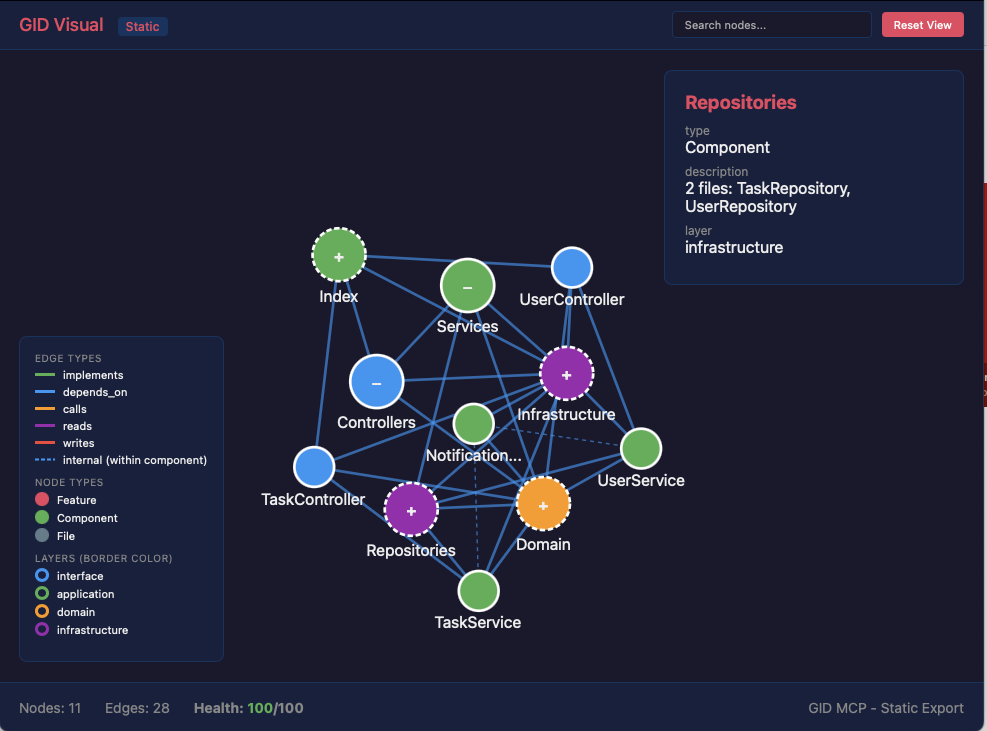
\includegraphics[width=\textwidth]{gid-visualization.png}
\caption{GID Visual: Interactive dependency graph visualization of a Task Management API. Nodes are color-coded by architectural layer (blue: interface, green: application, orange: domain, purple: infrastructure). Components can be expanded (+) to reveal internal file structure. The visualization shows 11 nodes and 28 edges with a health score of 100/100.}
\label{fig:gid-visual}
\end{figure}

\subsection*{Availability}

The GID specification and reference implementation are available as open source:

\begin{itemize}[noitemsep]
    \item Methodology: \url{https://github.com/tonioyeme/graph-indexed-development-principle}
    \item CLI Tool: \url{https://github.com/tonioyeme/graph-indexed-development-cli}
\end{itemize}

\section*{Acknowledgments}

The author thanks Wenying Deng for valuable discussions on graph theory concepts, causal inference principles, and mathematics notation that shaped the theoretical foundations of this work.

\bibliographystyle{plain}
\begin{thebibliography}{11}

\bibitem{c4model}
S. Brown, ``The C4 Model for Visualising Software Architecture,'' \url{https://c4model.com/}, 2018.

\bibitem{nygard2011}
M. Nygard, ``Documenting Architecture Decisions,'' Cognitect Blog, 2011.

\bibitem{eppinger2012}
S. D. Eppinger and T. R. Browning, \textit{Design Structure Matrix Methods and Applications}. MIT Press, 2012.

\bibitem{hogan2021}
A. Hogan et al., ``Knowledge Graphs,'' \textit{ACM Computing Surveys}, vol. 54, no. 4, 2021.

\bibitem{madge}
pahen, ``madge: Create graphs from your CommonJS, AMD or ES6 module dependencies,'' GitHub, 2023. \url{https://github.com/pahen/madge}

\bibitem{chen2021codex}
M. Chen et al., ``Evaluating Large Language Models Trained on Code,'' arXiv:2107.03374, 2021.

\bibitem{li2023starcoder}
R. Li et al., ``StarCoder: may the source be with you!'' arXiv:2305.06161, 2023.

\bibitem{zhang2023repocoder}
F. Zhang et al., ``RepoCoder: Repository-Level Code Completion Through Iterative Retrieval and Generation,'' arXiv:2303.12570, 2023.

\bibitem{fowler2002}
M. Fowler, \textit{Patterns of Enterprise Application Architecture}. Addison-Wesley, 2002.

\bibitem{martin2017}
R. C. Martin, \textit{Clean Architecture: A Craftsman's Guide to Software Structure and Design}. Prentice Hall, 2017.

\bibitem{depsrag2024}
M. Alhanahnah and Y. Boshmaf, ``DepsRAG: Towards Agentic Reasoning and Planning for Software Dependency Management,'' arXiv:2405.20455, 2024.

\end{thebibliography}

\end{document}
